 \chapter{Алгоритм классификации когнитивных состояний по данным фМРТ на основе метода межиндувидуальных корреляций}


\section{Формальная постановка задачи.}
\begin{annotation}
	Суть алгоритма: посмотреть какие воксели действуют схожим образом для каждого типа стимулов. Для этого применим метод Межиндивидуальных корреляций.
\end{annotation}

\subsection*{Основные Определения и Описание данных}

В работе используется несколько форматов представления данных:
\begin{compactitem}
	\item \texttt{NIfTI} --- файлы для результатов сегментации и удобного взаимодействия со средствами визуализации. Формат является адаптацией ранее использовавшегося формата \texttt{ANALYZE™} и обладает множеством преимуществ перед последним. Например поддержкой различных типов данных (точность от 8 до 128 бит)\,,хранением метаданных вместе с данными об объёме, возможностью хранить 4-d последовательности $(x,y,z,t)$  и проч. \cite{cox2004sort}. В данной работе подразумевается что данные разбиты покадрово и находятся в пронумерованных директориях соответствующих испытуемым.
	\item \texttt{HDF5} --- файлы использующиеся для хранения результатов промежуточных вычислений и <<кэширования>> данных для более удобной работы с ними.
\end{compactitem}

\section{Алгоритм определения информативных вокселей фМРТ}
\begin{annotation}
В данном разделе описывается алгоритм определения информативных вокселей. Применяются следующие подходы:
\begin{compactitem}
	\item Метод межиндивидуальных корреляций (ISC), состоящий в построении корреляционной матрицы для каждого вокселя для всех пар пациентов. Используется коэффициент корреляции Пирсона.
	\item Метод выделения t- статистики
	\item Обобщённая линейная модель.
\end{compactitem}
\end{annotation}

\subsubsection*{Метод межиндивидуальных корреляций (ISC)}


\ref{pic:cormat}


\begin{figure}
	\begin{subfigure}[b]{0.4\textwidth}
		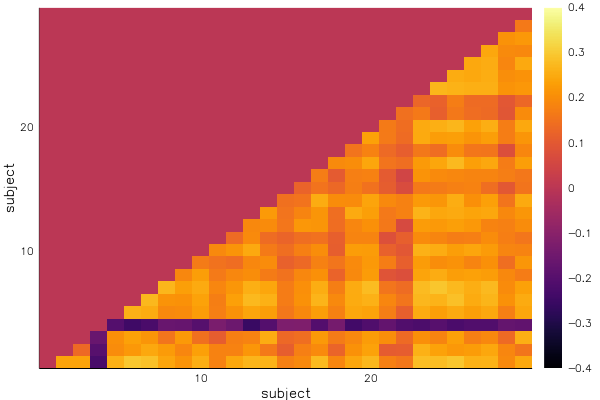
\includegraphics[width=\textwidth]{img/corisc.png}
		\caption{Информативного вокселя.}		
	\end{subfigure}
	\hfill
	\begin{subfigure}[b]{0.4\textwidth}
		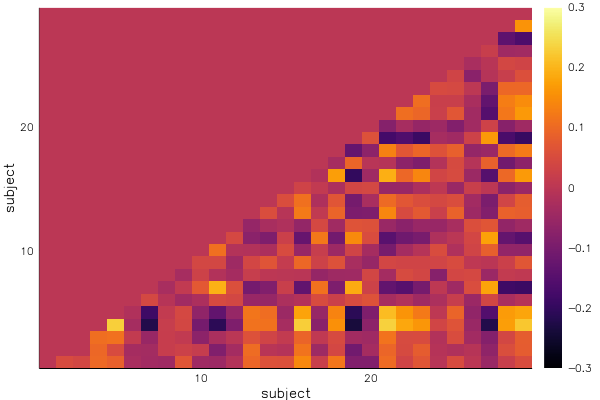
\includegraphics[width=\textwidth]{img/incisc.png}
		\caption{Неинформативного вокселя}
	\end{subfigure}
	\caption{Корреляционная матрица}
	\label{pic:cormat}
\end{figure}


\begin{figure}%
	\begin{center}
		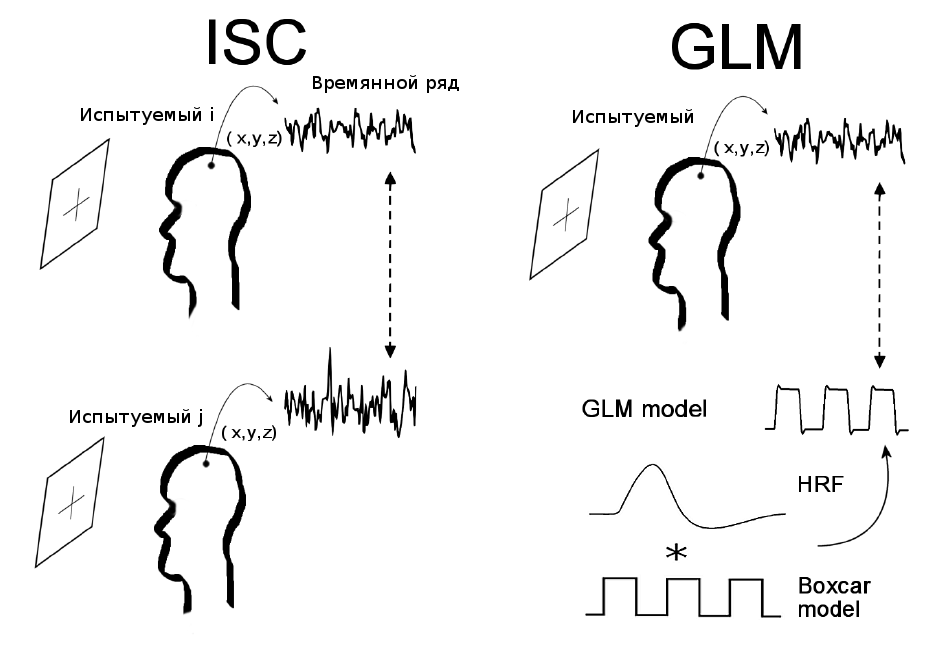
\includegraphics[width=.8\columnwidth]{./img/iscvsGLM.png}%
	\end{center}
	\caption{Сравнение принципов работы ISC и GLM}%
	\label{pic:iscvsglm}%
\end{figure}



\subsubsection*{Метод t-статистик}
В основе метода лежит предположение о том, что среднее значение информативных вокселей отличается 
во временных рядах, соответствующих различным стимулам. Напомним процедуру двухвыборочного t-критерия для независимых выборок\footnote{Выборки считаются независимыми так как в промежутках между стимулами пациент находится в состоянии покоя.}:
Пусть имеются две независимые выборки объемами ${\displaystyle n_{1}~,~n_{2}}$ нормально распределенных случайных величин ${\displaystyle X_{1},~X_{2}}$. Необходимо проверить по выборочным данным нулевую гипотезу равенства математических ожиданий этих случайных величин ${\displaystyle H_{0}:~M_{1}=M_{2}}$

Рассмотрим разность выборочных средних ${\displaystyle \Delta ={\overline {X}}_{1}-{\overline {X}}_{2}}$. Очевидно, если нулевая гипотеза выполнена ${\displaystyle \mathbb{M}(\Delta )=M_{1}-M_{2}=0}$ . Дисперсия этой разности равна исходя из независимости выборок: ${\displaystyle V(\Delta )={\frac {\sigma _{1}^{2}}{n_{1}}}+{\frac {\sigma _{2}^{2}}{n_{2}}}}$. Тогда используя несмещенную оценку дисперсии ${\displaystyle s^{2}={\frac {\sum _{t=1}^{n}(X_{t}-{\overline {X}})^{2}}{n-1}}}$  получаем несмещенную оценку дисперсии разности выборочных средних: ${\displaystyle s_{\Delta }^{2}={\frac {s_{1}^{2}}{n_{1}}}+{\frac {s_{2}^{2}}{n_{2}}}}$. Следовательно, t-статистика для проверки нулевой гипотезы равна

\begin{equation*}
{\displaystyle t={\frac {{\overline {X}}_{1}-{\overline {X}}_{2}}{\sqrt {{\frac {s_{1}^{2}}{n_{1}}}+{\frac {s_{2}^{2}}{n_{2}}}}}}}
\end{equation*}
Эта статистика при справедливости нулевой гипотезы имеет распределение ${\displaystyle t(df)}$, где \[{\displaystyle df={\frac {(s_{1}^{2}/n_{1}+s_{2}^{2}/n_{2})^{2}}{(s_{1}^{2}/n_{1})^{2}/(n_{1}-1)+(s_{2}^{2}/n_{2})^{2}/(n_{2}-1)}}}\]

\begin{figure}%
	\begin{center}
		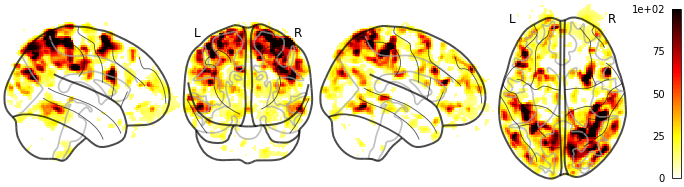
\includegraphics[width=.8\columnwidth]{./img/logpval.png}%
	\end{center}
	\caption{Сегментация с помощью \textit{t}-статистики\,($-log_{10}(P)$)}%
	\label{pic:ttest}%
\end{figure}



\section{Алгоритм формирования вектора характерных признаков сигналов фМРТ для классификации}
\begin{annotation}
Вектор признаков для классификатора формируется на основании результатов предыдущего шага с использованием метода главных компонент. Также убираются из рассмотрения признаки, не меняющиеся в зависимости от класса.
\end{annotation}

Полученные в ходу предыдущего шага $\mathbb{S}$ данные фильтруются с помощью экспериментально выбранных пороговых значений, мотивированных количеством признаков получаемых в ходу анализа. 
Функция принадлежности вокселя $(i,j,k)$ к множеству вокселей, значимых для классификации $(\mathcal{F})$, имеет вид:
\[
I((A_{i,j,k} > 0) \wedge (\mathbb{S}_{i,j,k} >  a) \wedge (\mathbb{CV} > b ) \wedge (\mathbb{M} .> 100))
\]
\section{Показатели точности классификации}
\begin{annotation}
	В качестве показателей точности используются:
	\begin{compactitem}
	\item Чувствительность ( ${ {SEN}}$ ) и специфичность ( ${ {SPE}}$ )
	\item $f1$ мера
	\end{compactitem}
\end{annotation}
Опишем формулы вычисления этих показателей:
\begin{empheq}{align*}
{ {SEN}}&={ {TP}}/P={ {TP}}/({ {TP}}+{ {FN}})\\
{ {SPE}}&={ {TN}}/N={ {TN}}/({ {TN}}+{ {FP}})\\
Precision&= {TP}/(TP+FP)\\
Recall&=TP/(TP+FN)\\
f1-measure &=  \sqrt{Precision\cdot Recall}\\
\end{empheq} 


\section{Формальное описание схемы применения алгоритма для классификации когнитивных состояний в режиме реального времени.}

\begin{annotation}
	В этой секции описывается применение алгоритма классификации к данным, поступающим с фМРТ-аппарата. Суть раздела: отображение фМРТ--снимку или небольшому набору снимков класса когнитивного состояния. ($\mathrm f (\mathbb N^3\to \mathbb R) \to Y$, где $Y$--конечный набор классов когнитивных состояний). 
\end{annotation}

\section{Выводы}

Был разработан алгоритм сегментации на основе коэффициента корреляции Пирсона, осуществляющий выделение значимых для классификации вокселей изображения при определённых допущениях о предварительной обработке данных и характере эксперимента. Он представляет собой упрощённый вариант алгоритма ISC, где выбор временного интервала осуществляется априорно, как выбор матрицы регрессоров в обобщённой линейной модели.

Также описан алгоритм сегментации с помощью двухвыборочного t-критерия. Он отличается от стандартного подхода дифференциацией вокселей на основе P-значения.

Для решения задачи сегментации также применен стандартный метод обобщённой линейной модели (GLM) в качестве контрольного. Используется его реализация в программном пакете SPM12.

Необходимо перечислить, какие теоретические результаты были получены с указанием степени новизны. Например: <<Была разработана такая-то модель. Она представляет собой адаптированную версию модели X, в которой уравнение Z заменено на уравнение Z'>>. Ещеfindmax(res) пример: <<Была предложена такая-то архитектура, она отличается от типовой в том-то и том-то. Это позволяет избежать таких-то проблем.>>. При этом следует заниматься <<высасыванием из пальца>>: <<Поставленная задача является типовой; для ее решения применены стандартные средства (перечислить, какие).>>.